\subsection{能耗、充电与时变碳排放核算}

在给定行驶速度下，电动车逐弧电耗与燃油车逐弧油耗写为距离和载重的函数：
\begin{align}
e^E_{ij,k}&=(\alpha_{0k}^E+\alpha_{1k}^E L_{ir})d_{ij}, && k\in K^E,\label{eq:ev-energy}\\
f^F_{ij,k}&=(\alpha_{0k}^F+\alpha_{1k}^F L_{ir})d_{ij}, && k\in K^F.\label{eq:cv-fuel}
\end{align}
其中，最终稿仍需逐式核对系数的单位、实现值和文献来源\cite{ref:goeke-2015}。

设充电会话$q$发生于站点$s(q)$，功率为$P_{s(q)}$，其与电网时段$t$的重叠时长为
\begin{equation}
g_{qt}=\left[\min\{h_q+\Delta_q,\bar T_t\}-\max\{h_q,\underline T_t\}\right]_+,
\label{eq:charge-overlap}
\end{equation}
则时段充电量为$y_{qt}=P_{s(q)}g_{qt}/60$，并满足$\sum_{t\in T}y_{qt}=Y_q$。部分充电和公共站容量的处理参照相关电动车路径研究\cite{ref:froger-2022,ref:keskin-2016}。

实体车排班模式$p$的燃油车直接排放和电动车充电侧间接排放分别为
\begin{align}
E_{kp}^{F}&=\lambda^F\sum_{r\in\mathcal R_{kp}}\sum_{(i,j)\in r}f^F_{ij,k},\label{eq:cv-emission}\\
E_{kp}^{E}&=\sum_{q\in\mathcal Q_{kp}}\sum_{t\in T}\gamma_ty_{qt}.\label{eq:ev-emission}
\end{align}
系统全口径排放为
\begin{equation}
E^{\mathrm{sys}}=\sum_{k\in K}\sum_{p\in\Omega_k}(E_{kp}^{F}+E_{kp}^{E})z_{kp}.
\label{eq:system-emission}
\end{equation}
式\eqref{eq:system-emission}是后文各决策层共同使用的排放尺：移动充电开始时刻改变$y_{qt}$的时段分布，改变车型指派改变直接与间接排放的构成，动态重规划则改变车辆可用时刻和充电窗口。

\subsection{目标函数与约束}

运营成本由实体车固定成本、里程成本、燃油成本和充电电费构成：
\begin{equation}
C^{\mathrm{op}}=\sum_{k\in K}c_k^{\mathrm{fix}}u_k+
\sum_{k\in K}\sum_{p\in\Omega_k}\left(c_k^{\mathrm{km}}D_{kp}+p^FF_{kp}+
\sum_{q\in\mathcal Q_{kp}}\sum_{t\in T}p^e_{s(q),t}y_{qt}\right)z_{kp}.
\label{eq:operation-cost}
\end{equation}
固定成本按启用实体车计取：
\begin{equation}
u_k=\sum_{p\in\Omega_k}z_{kp},\qquad \sum_{p\in\Omega_k}z_{kp}\leq 1.
\label{eq:vehicle-use}
\end{equation}
采用单位碳价把排放纳入统一货币目标：
\begin{equation}
\min Z=C^{\mathrm{op}}+p^{\mathrm{car}}E^{\mathrm{sys}}.
\label{eq:objective}
\end{equation}

每个客户由一个实体车排班模式恰好覆盖：
\begin{equation}
\sum_{k\in K}\sum_{p\in\Omega_k}A_{ikp}z_{kp}=1,\qquad i\in N.
\label{eq:coverage}
\end{equation}
模式内部满足流守恒、载重与硬时间窗约束：
\begin{align}
\sum_jx_{ijr}&=\sum_jx_{jir}=a_{ir}, && i\in N,\label{eq:flow}\\
0\leq L_{ir}&\leq Q_k,\qquad L_{jr}\leq L_{ir}-q_j+M(1-x_{ijr}),\label{eq:load}\\
e_i a_{ir}&\leq T_{ir}\leq l_i+M(1-a_{ir}),\nonumber\\
T_{jr}&\geq T_{ir}+s_i+t_{ij}-M(1-x_{ijr}).\label{eq:time-window}
\end{align}
电动车电量沿弧传播，并仅在允许地点补能：
\begin{equation}
b_k^{\min}\leq b_{ir}\leq B_k,\qquad
b_{jr}\leq b_{ir}+Y_{ir}-e^E_{ij,k}+M(1-x_{ijr}),\quad k\in K^E.
\label{eq:soc}
\end{equation}
同一实体车相邻趟$r\rightarrow r'$满足时间与电量连续：
\begin{align}
T_{d^+_{r'}r'}&\geq T_{d^-_rr}+\sum_{q\in\mathcal Q_{kp}^{rr'}}\Delta_q,\label{eq:trip-time}\\
b_{d^+_{r'}r'}&=b_{d^-_rr}+\sum_{q\in\mathcal Q_{kp}^{rr'}}Y_q.\label{eq:trip-energy}
\end{align}
公共站容量约束为
\begin{equation}
\sum_{k\in K}\sum_{p\in\Omega_k}O_{skpt}z_{kp}\leq C_s,\qquad s\in S,\ t\in T.
\label{eq:station-capacity}
\end{equation}
式\eqref{eq:station-capacity}不施加于车场充电。

设第$m$次重规划时刻为$\tau_m$，待服务客户集合按事件更新：
\begin{equation}
N^{\tau_m}=\left(N^{\tau_{m-1}}\setminus N_{\mathrm{served}}^{\tau_m}\setminus N_{\mathrm{cancel}}^{\tau_m}\right)\cup N_{\mathrm{new}}^{\tau_m}.
\label{eq:dynamic-set}
\end{equation}
已经发生的成本与排放分别累计为
\begin{equation}
\bar C^{\tau_m}=\bar C^{\tau_{m-1}}+\Delta C^{\tau_{m-1}},\qquad
\bar E^{\tau_m}=\bar E^{\tau_{m-1}}+\Delta E^{\tau_{m-1}}.
\label{eq:dynamic-account}
\end{equation}
新一轮优化仅计算剩余问题，已执行前缀作为不可撤销约束。

\section{算法设计}

\subsection{算法框架}

GCI-DMM-VRP同时包含路径、车型、实体车多趟、充电和动态状态继承。本文采用成熟混合遗传搜索作为搜索底座，在其上组织一条面向本问题的串行改进链\cite{ref:vidal-2012,ref:wouda-2024}。底座本身不作为算法创新，问题特化组件的贡献仍需被接受的正式证据检验。

框架坚持“唯一一本账”：候选是否被接受、能否进入种群、能否存活以及能否被选为父代，均由同一完整评价器给出的完整成本与完整可行性决定。能源消耗、充电、跨趟时间---电量衔接、时变电价和时变碳强度进入同一本账。候选完成失败保留失败原因，不静默冒充初始解。

\begin{figure}[htbp]
  \centering
  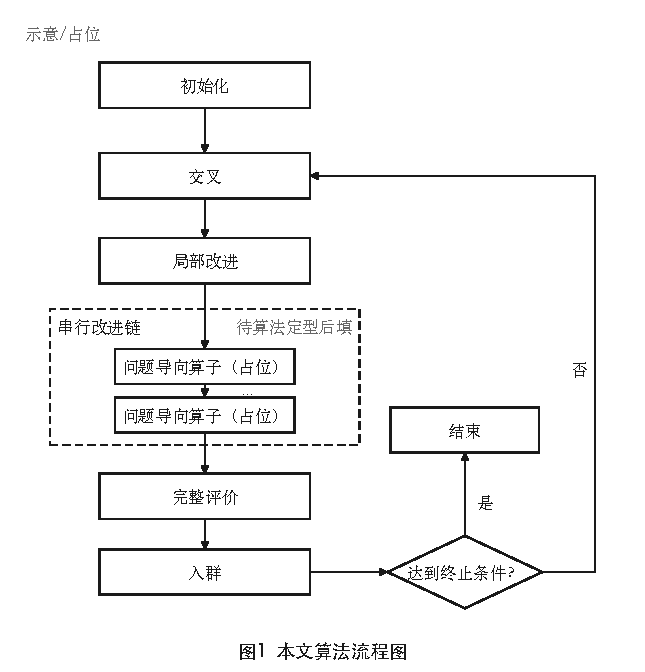
\includegraphics{figures/figure_1_algorithm_flow.pdf}
  \refstepcounter{figure}
  \label{fig:algorithm-flow}
\end{figure}

\subsection{算法步骤}

\textbf{步骤一：构造状态快照与可行起点。} 静态阶段读取订单、车场、有限实体车队和碳强度序列；动态阶段读取式\eqref{eq:dynamic-set}--\eqref{eq:dynamic-account}定义的剩余客户与车辆状态。初始个体先经完整模型检查。

\textbf{步骤二：执行混合遗传搜索主循环。} 算法维护可行与不可行子种群，通过选择、交叉、教育与多样性管理更新候选，罚系数按可行解比例调整。停止条件和预算由本项目收敛记录标定，不直接照搬其他算法的迭代数。

\textbf{步骤三：施加问题特化动作。} 便宜代理只提名有界候选，完整真值逐项评价并决定是否接受。\TBD{算法定稿后列出进入论文的特化动作与出处}。

\textbf{步骤四：完成实体车排班与充电。} 将配送趟分配给具体实体车，按时间顺序衔接多趟并补齐电量、充电会话、分时电价和碳排放。违反时间窗、容量、电量、公共站容量或实体车上限的候选保留失败原因。

\textbf{步骤五：入群、生存与父代选择。} 入群按完整可行性分池，生存选择和父代选择使用同一完整账；全局最好解必须完整可行。

\textbf{步骤六：独立验解与动态调用。} 进入种群的候选重新执行独立检查，只有完整可行且严格改善的候选更新最好解。事件触发后冻结已经执行的路径前缀，更新车辆状态，再求解剩余问题。

\section{数值实验设计与算法有效性}

\subsection{算例与参数}

代表实例为京津冀50客户、2车场、97个公共站节点的构造算例，客户责任按编号等分为两家企业各25个。动态事件流包含10个新增客户事件，接单窗为08:00--10:00，共5个触发批；分时电价和碳强度的信息分辨率为1小时。

车辆成本、容量与柴油价格取自本文算例的车辆参数与当地价格表；电动车非能源里程成本中的电池折旧部分按电池价格与寿命里程折算，寿命里程参照Goeke与Schneider\cite{ref:goeke-2015}，电动车相对燃油车每辆每日50元的固定成本溢价参照陈婉茹等\cite{ref:chen-wanru-2023}；车场单车额定充电功率参照中国地方新能源汽车充（换）电设施专项规划；分时电价与逐时电网碳强度取自北京2025年2月12日的当地价格表与省级逐小时碳强度投影数据集，信息分辨率为1小时。尚未闭合到原始页码的出处为\TBD{出处或页码}。关键参数如表\ref{tab:parameters}所示。

\begin{table}[htbp]
  \centering
  \caption{关键车辆、充电、电价与碳强度参数及来源}
  \label{tab:parameters}
  \scriptsize
  \begin{tabular}{lrl}
    \toprule
    参数 & 数值 & 单位\\
    \midrule
    燃油车日固定成本 & 170.00 & 元/(辆·日)\\
    电动车日固定成本 & 220.00 & 元/(辆·日)\\
    燃油车非能源里程成本 & 0.7800 & 元/km\\
    电动车非能源里程成本 & 0.9145 & 元/km\\
    车辆容积容量 & 7.2 & m$^3$\\
    柴油价格 & 7.48 & 元/L\\
    车场单车额定充电功率 & 60.0 & kW\\
    车场分时电价（谷/平/峰） & 0.5633／0.8364／1.1486 & 元/kWh\\
    公共站服务费 & 0.4 & 元/kWh\\
    公共站分时总电价（谷/平/峰） & 0.9633／1.2364／1.5486 & 元/kWh\\
    逐时电网碳强度（24 个小时值） & 0.1541～0.6439 & kgCO$_2$e/kWh\\
    单位碳价 & 0.07502 & 元/kgCO$_2$e\\
    \bottomrule
  \end{tabular}
\end{table}
